\documentclass[11pt,a4paper]{article}
\usepackage[a4paper, margin=3cm]{geometry}

\usepackage{natbib}
\usepackage{charter} % Use the Charter font
\usepackage[utf8]{inputenc} % Use UTF-8 encoding
\usepackage{microtype} % Slightly tweak font spacing for aesthetics
\usepackage[english, spanish, es-nodecimaldot]{babel} % Language hyphenation and typographical rules
\usepackage{amsthm, amsmath, amssymb} % Mathematical typesetting
\usepackage{float} % Improved interface for floating objects
\usepackage[]{threeparttable}
\usepackage[]{booktabs}
\usepackage{enumerate}
\usepackage[T1]{fontenc}
\usepackage{makecell}
\usepackage{adjustbox}

\title{\bf Taller 1: Predicting Income \\ Big data and Machine learning for Economics}

\author{Alison Gissell Ruiz Ruiz - Código 202116230\\ 
Daniel Delgado - Código\\
José Julián Parra Montoya - Código 202213144 }
\date{}

\begin{document}

\maketitle

\section{Descripción de los datos}

La Gran Encuesta Integrada de Hogares (GEIH) es una encuesta recolectada por el DANE de manera mensual, que busca aportar insumos para el análisis del mercado laboral. Se busca desarrollar una predicción del ingreso de una persona dada ciertas características, esto podría ser de utilidad para evitar fraude en reportes de ingresos y pagos de impuestos, se busca adicional realizar un modelo que represente la relación entre las ganancias y la edad de las personas, así como la relación entre las ganancias y el género, con el fin de analizar la brecha salarial que podrían o no tener las personas de género femenino con respecto al masculino. \\

En este caso se utiliza la encuesta realizada en 2018 restringida a individuos mayores de 18 años. Para el análisis que se busca realizar se requieren determinar una(s) variables(s) que midan adecuadamente los \emph{earnings} (ganancias) y el \emph{income} (ingreso). 
En economía laboral ambas cosas son conceptualmente diferentes: mientras que las ganancias corresponden al salario o ingresos laborales, el ingreso fuentes distintas al factor trabajo como las ganancias de capital CITA. Los datos empleados fueron obtenidos mediante \emph{webscrapping}, método que facilita la extracción de información de páginas web. El código de obtención de información y el desarrollo de los algoritmos previamente descritos se desarrollan empleando \emph{R} como leguaje de programación.
\\

Para medir \emph{earnings} se emplea el ingreso laboral (\textit{y\_ingLab\_m} en la GEIH). De acuerdo a una exploración previa de los datos, esta variable se puede calcular de dos formas: en primer lugar, como la suma de los salarios 
percibidos por las ocupaciones primarias (\textit{y\_salary\_m}) y secundarias (\textit{y\_salarySec\_m}), beneficios laborales como auxilio de transporte (\textit{y\_auxilioTransp\_m}), auxilio de vivienda (\textit{y\_vivienda\_m}), viaticos (\textit{y\_viaticos\_m}), salarios en especie (\textit{y\_especie\_m}), 
bonificaciones (\textit{y\_bonificaciones\_m}) y la proporción mensual de los diferentes tipos de prima. Otra alternativa es mediante la suma del ingreso percibido por la ocupación primaria (\textit{impa}) y secundaria (\textit{isa}) pero excluyendo los montos mensuales de subsidios alimenticios (\textit{y\_auxilioAliment\_m}) y subsidios por accidentes (\textit{y\_accidentes\_m}), así como las ganancias de los trabajadores cuenta propia (\textit{y\_gananciaNeta\_m}). Esta variable es más apropiada que simplemente el salario (\textit{y\_salary\_m}) para medir \emph{earnings} ya que captura también los ingresos laborales de ocupaciones secundarias, cosa que no hace la primera.\\

Para medir \emph{income} se utilizará el ingreso total (\textit{ingtot}). Esta variable, además de incluir el ingreso laboral, contempla las ganancias de los trabajadores cuenta propia, los ingresos por arrendamientos e intereses (\textit{iof6}), jubilaciones y pensiones (\textit{iof2}), 
transferencias monetarias (\textit{iof3i} y \textit{iof3h}), y el ingreso de los desocupados o inactivos (\textit{imdi}). 
Un hecho ampliamente documentado en las encuestas de hogares es que las características de los individuos explican el patrón de datos faltantes en las variables de ingreso CITA. Esto indica que no es apropiado omitir los datos faltantes pues esto sesgaría la distribución
de ingresos en los análisis posteriores. En la investigación de \cite{imputacionGEIH}, encuentran que el método de imputación óptimo para la GEIH es el método Hot Deck. De acuerdo a la descripción metodológica del DANE, el proceso de imputación de las variables de ingreso ya fue realizado, y estas variables
se representan en la base con el sufijo \emph{es} (\textit{impaes} para la imputación de la variable \textit{impa} o ingreso de la ocupación principal, etc.). En el cuadro \ref{tbl:DatosFaltantes} se presenta un conteo de los datos faltantes en las variables de Ingreso Laboral e Ingreso Total.


\begin{table}[H]
  \centering
  \caption{Datos faltantes} 
  \label{tab:missing}
  \begingroup\fontsize{9pt}{10pt}\selectfont
  \begin{tabular}{lrr}
    \hline
  \addlinespace
    & Faltantes & Total \\
  \addlinespace
   \hline
   Ingreso Total &   0 & 24568 \\ 
    Ingreso Laboral & 14676 & 24568 \\ 
    Ingreso Laboral Imputado & 4872 & 24568 \\ 
     \addlinespace
  \hline
  \addlinespace
  \end{tabular}
  \endgroup
  \label{tbl:DatosFaltantes}
  \end{table}
  

Como puede observarse, no existen datos faltantes en el Ingreso Total. Esto se debe a que esta variable corresponde a la suma de las variables descritas previamente teniendo en cuenta, en cada caso, la versión de la variable donde fue necesario realizar la imputación,
de manera que esta variable, al ser suma de variables imputadas, ya se encuentra imputada. En el caso del Ingreso Laboral, se observa que existen datos faltantes; no obstante, algunos de sus componentes como los ingresos de las ocupaciones primaria y secundaria fueron imputados por el DANE, de manera que se pueda reducir la cantidad de datos faltantes
aprovechando esta imputación al sustraer las variables adecuadas (como la ganancia de los independientes, el auxilio por accidente y el auxilio alimenticio).
En la última fila del cuadro \ref{tbl:DatosFaltantes} se muestra la variable con la corrección. Los demás datos faltantes consisten en casos donde el individuo es un trabajador por cuenta propia para el cual no es posible determinar qué parte de sus ganancias corresponde a ingresos laborales, quedando en total 4872 datos donde no es posible realizar imputación sin sesgar los datos.\\

El cuadro \ref{tbl:estadisticasDesc} contiene algunas estadísticas descriptivas para estas variables. Como puede observarse, tras utilizar la imputación del DANE para el Ingreso Laboral se obtiene una distribución a la izquierda de la distribución de Ingreso Total pues la media, la mediana y el percentil 90 son inferiores a los de esta última. 
Esto es de esperarse pues el Ingreso Total contiene al Ingreso Laboral junto a otros tipos de ingresos, lo que debería producir valores más grandes para cada individuo. De no utilizarse los valores imputados, como puede observarse en la tercera fila, se tendria una distribución de Ingreso Laboral a la derecha de la distribución de Ingreso Total, lo cual es conceptualmente incorrecto.


\begin{table}[H]
  \centering
  \caption{Estadísticas descriptivas variables dependientes} 
  \label{tab:descriptive_dependent}
  \begingroup\fontsize{9pt}{10pt}\selectfont
  \begin{tabular}{lrrrr}
    \hline
  \addlinespace
    & Media & Mediana & D.E. & Percentil 90 \\
  \addlinespace
   \hline
   Ingreso total & 1369323.55 & 900000.00 & 2387364.35 & 2921931.33 \\ 
    Ingreso laboral & 1745416.34 & 1032559.84 & 2403441.13 & 3250000.00 \\ 
    Ingreso Laboral Imputado & 1008801.19 & 737717.00 & 2033436.79 & 2166666.75 \\ 
     \addlinespace
  \hline
  \addlinespace
  \end{tabular}
  \endgroup
  \label{tbl:estadisticasDesc}
  \end{table}

 Las variables que se utilizarán para predecir los ingresos descritos previamente son: la edad (\textit{age}), la pertenencia al género femenino (\textit{female}), la tenencia de educación universitaria (\textix{college\_2}), la condición de ser trabajador cuenta propia (\textit{cuentaPropia}), la condición de informalidad (\textit{informal})  y el oficio (\textit{oficio}). 
 En el cuadro \ref{tbl:estadisticasDescInd} se presentan algunas estadísticas descriptivas. Este indica que la edad, que es un variable numérica, es en promedio de 42 años y que la distribución es aproximadamente simétrica pues la mediana (20 años) está cerca a la media. Así mismo se observa que la edad más común es de 23 años, y que existe, en promedio, una desviación de 17 años respecto a la media. 
A diferencia de la edad, la condición de ser mujer, de tener educación universitaria, ser cuenta propia o trabajador informal son todas variables dicótomas. El promedio de las variables dicótomas indica la frecuencia con que la condición descrita por la variable se encuentra en la muestra. Por lo tanto, el 53\% de los individuos son mujeres, el 30\% tiene educación universitaria, el 21\% es trabajador por cuenta propia, y el 59 \% es formal; estas frecuencias son consistentes con las modas de cada distribución. 
Finalmente, el oficio es una variable multinomial; la categoría ocupacional más común es la 45, que consiste en vendedores ambulantes o a domicilio. Se debe notar que la variable de educación universitaria es una variable nueva que debió calcularse debido a que la variable de educación universitaria existente en la base de datos (\textit{college}) no refleja en realidad el nivel de educación superior si no el nivel de educación media. 

\begin{table}[htp]
  \centering
  \caption{Estadísticas descriptivas variables independientes} 
  \label{tab:descriptive_independent}
  \begingroup\fontsize{9pt}{10pt}\selectfont
  \begin{tabular}{lrrrr}
    \hline
  \addlinespace
    & Media & Mediana & Moda & D.E. \\
  \addlinespace
   \hline
   Edad & 42.31 & 40.00 & 23.00 & 17.27 \\ 
    Mujer & 0.53 &  & 1.00 &  \\ 
    Universidad & 0.40 &  & 0.00 &  \\ 
    Cuenta Propia & 0.21 & & 0.00 &  \\ 
    Formal & 0.59 & & 1.00 & \\ 
    Oficio &  & 45.00 & &  \\ 
     \addlinespace
  \hline
  \addlinespace
  \end{tabular}
  \endgroup
  \label{tbl:estadisticasDescInd}
  \end{table}
  
  En el cuadro \ref{tbl:oficiosComunes} se presentan las 10 categorías ocupacionales más comunes. Estas incluyen vendedores ambulantes (oficio código 45), axiliares de oficina o bodega (39), conductor de vehículo (98), empleada doméstica (54) y cocinero o camarero (53). Algo común de estas profesiones es su alto grado de informalidad, lo cual es consistente con la frecuencia de informales que se encuentró previamente.

    \begin{table}[H]
      \centering
      \caption{Oficios más comunes} 
      \label{tab:oficios_freq}
      \begingroup\fontsize{9pt}{10pt}\selectfont  
    \begin{tabular}{ccc}
      \hline
      Oficio & Conteo & \%\\
      \hline
      45 & 1763 & 0.11\\
      39 & 955 & 0.06\\
      98 & 831 & 0.05\\
      54 & 771 & 0.05\\
      53 & 704 & 0.04\\
      21 & 693 & 0.04\\
      41 & 662 & 0.04\\
      58 & 659 & 0.04\\
      95 & 622 & 0.04\\
      55 & 610 & 0.04\\
      \hline
      \end{tabular}   
      \endgroup
      \label{tbl:oficiosComunes}
    \end{table}

    Ahora resulta interesante analizar la relación entre las variables dependientes y algunas de las variables independientes.
    En los cuadros \ref{tbl:mediasIndA} y \ref{tbl:mediasIndB} se realizan pruebas de diferencia de medias para ambos tipos de ingresos agrupados por algunas características de los individuos. Los hallazgos del cuadro \ref{tbl:mediasIndA} resultan sorprendentes: en las columnas 1 y 2 se 
    puede observar que el ingreso total promedio para las mujeres es de \$1'144.787 mientras que para los hombres es de \$1'622,191, y la diferencia entre ambos promedios en todos los casos es estadísticamente significativa (columna 3). 
    Algo similar sucede con los ingresos laborales, los cuales son en promedio de \$830,259 para las mujeres y de \$1'232,013 para los hombres; nuevamente la diferencia entre ambos promedios, para los dos tipos de ingresos, es estadísticamente significativa.
    En los individuos con estudios universitarios se observa el mismo patrón: tanto su ingreso total promedio (\$2'210,500) como su ingreso laboral promedio (\$1'701,006) es superior respecto a aquellos que no poseen estudios universitarios (818,004 y 526,196 respectivamente).
    La diferencia entre ambos promedios es nuevamente estadísticamente significativa.
    
      \begin{table}[H]
        \centering
        \caption{Diferencia de medias variables independientes (A)} 
        \label{tab:dif_medias_a}
%        \begingroup\fontsize{9pt}{10pt}\selectfont
        \resizebox{\textwidth}{!}{
        \begin{tabular}{ccccccc}
        \toprule
        \multicolumn{1}{c}{ } & \multicolumn{2}{c}{Mujer} & \multicolumn{1}{c}{} & \multicolumn{2}{c}{Universitario} & \multicolumn{1}{c}{} \\
        \cmidrule(l{3pt}r{3pt}){2-3} \cmidrule(l{3pt}r{3pt}){5-6}
        & \makecell[c]{Media Sí\\(1)} & \makecell[c]{Media No\\(2)} & \makecell[c]{Diferencia\\(3)} & \makecell[c]{Media Sí\\(4)} & \makecell[c]{Media No\\(5)} & \makecell[c]{Diferencia\\(6)}\\
        \midrule
        Ingreso total  & 1144787.68 & 1622191.16 & -477403.48*** & 2210500.86 & 818004.12 & 1392496.74***\\
         & (1945185.64) & (2781507.32) & {}[30989.16] & (3462752.02) & (899429.22) & {}[35877.96]\\
       Ingreso laboral  & 830259.7 & 1232013.76 & -401754.06*** & 1701006.24 & 526196.2 & 1174810.04***\\
         & (1829872.41) & (2242514.38) & {}[29673.55] & (2936768.86) & (661870.04) & {}[33221.98]\\
         \bottomrule
        \end{tabular}
        }
        \begin{tablenotes}[para,flushleft]
          \centering \footnotesize Nota: desviaciones estándar en paréntesis y erores estándar en paréntesis cuadrados.  ***p<0.01, **p<0.05, *p<0.1.            
      \end{tablenotes}
      \label{tbl:mediasIndA}
        \end{table}

      En el cuadro \ref{tbl:mediasIndB} se observa el comportamiento de los ingresos según algunas características de los trabajadores. En la columna 1 se observa que el ingreso total de los trabajadores cuenta propia
      es de \$1'386,842 y su ingresos laboral es de \$1'077,734. Esto no es tan distinto al ingreso total promedio de los trabajadores que no son cuenta propia \$1'364,727 y a su ingreso laboral promedio \$1'006,204, como se observa en la columna 2.
      En efecto la diferencia entre ambos tipos de promedios no es estadísticamente significativa (columna 3). Una posible explicación de esto es que las características que explican los mayores ingresos vistas hasta ahora (como el género y el nivel educativo) estén distribuidas de forma homogénea entre ambos tipos de trabajadores.
      Este patrón no se sostiene para los informales, quienes tienen ingresos totales y laborales en promedio inferiores (\$944,022 y \$786,169, respectivamente) a los de los trabajadores no informales (\$2'350,537 y \$2'058,596); la diferencia entre ambos promedios, para ambos tipos de ingresos, es estadísticamente significativa, como es de esperarse. 


        \begin{table}[H]
          \centering
          \caption{Diferencia de medias variables independientes (B)} 
%          \begingroup\fontsize{9pt}{10pt}\selectfont  
          \label{tab:dif_medias_b}
          \resizebox{\textwidth}{!}{
          \begin{tabular}{cccccccc}
          \toprule
          \multicolumn{1}{c}{ } & \multicolumn{2}{c}{Cuenta Propia} & \multicolumn{1}{c}{} & \multicolumn{2}{c}{Informal} & \multicolumn{1}{c}{} \\
          \cmidrule(l{3pt}r{3pt}){2-3} \cmidrule(l{3pt}r{3pt}){5-6}
           & \makecell[c]{Media Sí\\(1)} & \makecell[c]{Media No\\(2)} & \makecell[c]{Diferencia\\(3)} & \makecell[c]{Media Sí\\(4)} & \makecell[c]{Media No\\(5)} & \makecell[c]{Diferencia\\(6)}\\
          \midrule
          Ingreso total  & 1386842.09 & 1364727.43 & 22114.66 & 944022.72 & 2350537.97 & -1406515.25***\\
           & (2054585.85) & (2467277.18) & {}[33756.84] & (1181637.68) & (3224865.87) & {}[35716.23]\\
         Ingreso laboral  & 1077734.94 & 1006204.51 & 71530.43 & 786169.2 & 2058596.77 & -1272427.57***\\
           & (1573625.11) & (2048728.94) & {}[60699.94] & (1121024.92) & (2666218.2) & {}[35080.94]\\          
          \bottomrule
          \end{tabular}
          }
          \begin{tablenotes}[para,flushleft]
            \centering \footnotesize Nota: desviaciones estándar en paréntesis y erores estándar en paréntesis cuadrados.  ***p<0.01, **p<0.05, *p<0.1.            
        \end{tablenotes}
        \label{tbl:mediasIndB}
          \end{table}



          
          Finalmente, en la figura \ref{fig:ingresos_edad} se muestra el comportamiento de los ingresos laborales y totales promedio por intervalo de edad. Para el ingreso laboral se observa un patrón inicialmente creciente hasta los 45 años; posteriormente comienza a decrecer hasta que es nulo para los individuos mayores a 90 años. Este patrón se asemeja al encontrado para el ingreso total, aunque en este caso el ingreso total para los individuos mayores a 45 años decrece de forma mucho más suave. Esto se debe a los programas de seguridad social y transferencias monetarias a personas de la tercera edad, los cuales garantizan un nivel de ingreso mínimo en la vejez.

\begin{figure}[H]
    \centering
        \caption{Ingresos por intervalo de edad}
    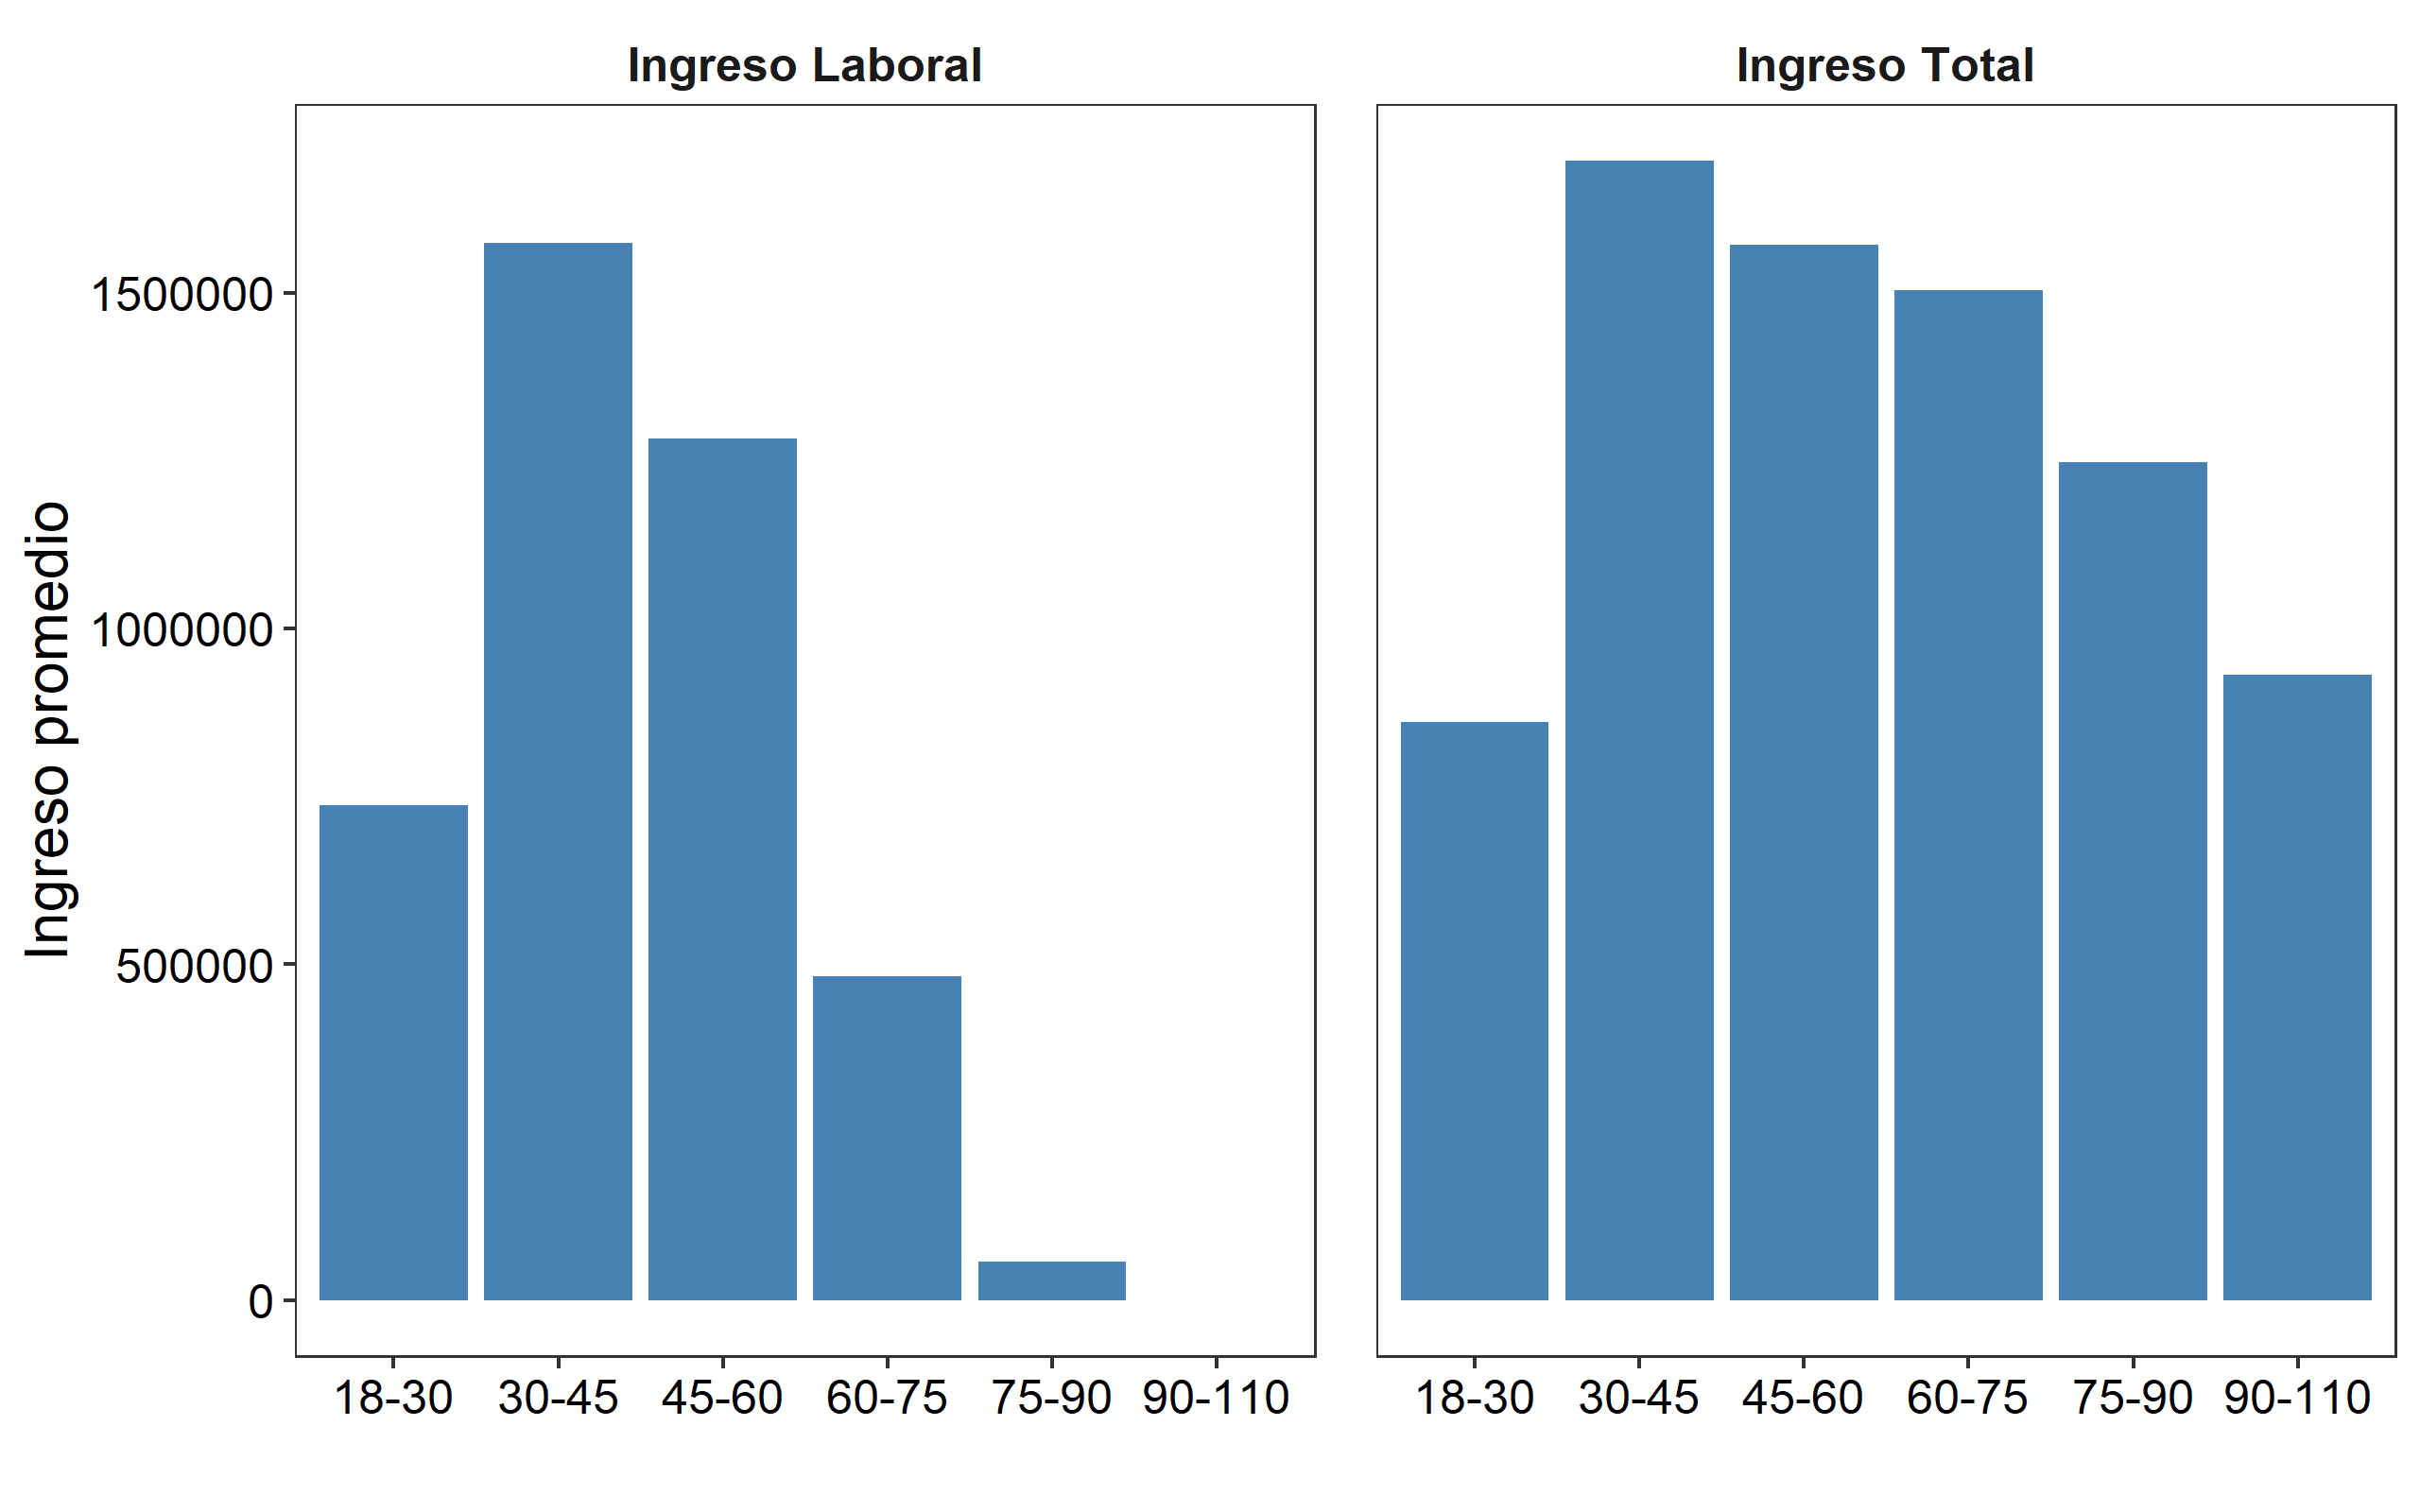
\includegraphics[width=\textwidth]{../views/ingresos_edad.png}
    \label{fig:ingresos_edad}
\end{figure}

\section{Análisis de predicción para \emph{earnings}}

En esta sección se busca la especificación que permita generar la mejor predicción del ingreso laboral.
En el cuadro \ref{tbl:earningsEspecif} se muestran las diferentes especificaciones empleadas, las cuales utilizan las características de los individuos descritas en la primera sección.

\begin{table}[H]
  \centering
  \caption{Especificaciones para la predicción de \emph{earnings}}
  \label{tab:model_specification_pred}
  \resizebox{\textwidth}{!}{
  \begin{tabular}{@{}ll@{}}
  \toprule
  Modelo & Especificación \\ \midrule
  1 & $IngresoLaboral=\beta_0+\beta_1\,Edad+\beta_2\,Edad^2+e_1$ \\
  2 & $Log(IngresoLaboral+1)=\beta_0+\beta_1\,Mujer+e_2$\\
  3 & $IngresoLaboral=\beta_0+\beta_1\,Edad+\beta_2\,Edad^2+\beta_3\,Mujer+e_3$  \\
  4 & $IngresoLaboral=\beta_0+\beta_1\,Edad+\beta_2\,Edad^2+\beta_3\,Mujer+\beta_4\,CuentaPropia+e_4$ \\
  5 & $IngresoLaboral=\beta_0+\beta_1\,Edad+\beta_2\,Edad^2+\beta_3\,Mujer+\beta_4\,CuentaPropia+\beta_5\,Universitario+e_5$\\
  6 & $IngresoLaboral=\beta_0+\beta_1\,Edad+\beta_2\,Edad^2+\beta_3\,Mujer+\beta_4\,CuentaPropia+\beta_5\,Universitario+\beta_6\,Formal+e_6$\\
  7 & $IngresoLaboral=\beta_0+\beta_1\,Edad+\beta_2\,Edad^2+\beta_3\,Mujer+\beta_4\,CuentaPropia+\beta_5\,Universitario+\beta_6\,Formal+\beta_7\,Formal*Universitario+e_7$  \\
  8 & $IngresoLaboral=\beta_0+\beta_1\,Edad+\beta_2\,Edad^2+\beta_3\,Mujer+\beta_4\,CuentaPropia+\beta_5\,Universitario+\beta_6\,Formal+\beta_7\,Formal*Universitario+\alpha'Oficio+ e_8$ \\ 
  \bottomrule
  \end{tabular}
  }
  \begin{tablenotes}[para,flushleft]
    \centering \footnotesize Nota: $\alpha$ es un vector de parámetros que contiene los parámetros de cada una de las variables dicótomas que se pueden crear a partir de la variable multinomial de oficios. Así mismo, ``Oficio'' es un vector de variables dicótomas. Para la estimación de todas las especificaciones fue necesario descartar la categoría 78 de oficio a la cual solo correspondía un individuo en la muestra.
\end{tablenotes}
\label{tbl:earningsEspecif}
  \end{table}

La Raíz Cuadrada del Error Cuadrático Medio (RMSE) de todas las especificaciones se reporta en el cuadro \ref{tbl:RMSEearnings}. Esta métrica de desempeño fue escogida pues penaliza de forma creciente los errores lo cual es deseable al estimar un ingreso (los errores de predicción más grandes son más problemáticos); así mismo, permite obtener los errores en las unidades de medida originales de la variable.    

\begin{table}[H]
  \centering
  \caption{RMSE para diferentes especificaciones de \emph{earnings}}
  \label{tab:rmse_punto4}
  \begin{tabular}{@{}ll@{}}
  \toprule
  Modelo & RMSE \\ \midrule
  1 & 155183853 \\
  2 & 166030377 \\
  3 & 154976001 \\
  4 & 154390798 \\
  5 & 144029580 \\
  6 & 143075426 \\
  7 & 142393393 \\
  8 & 134801931 \\ \bottomrule
  \end{tabular}
  \label{tbl:RMSEearnings}
  \end{table}


Como puede observarse, la mejor especificación es la dada por el modelo 8 pues esta arroja el RMSE más bajo. La segunda mejor es la dada por el modelo 7. 
Ahora se procederá a hacer un análisis de las observaciones más influyentes. Para esto se emplea el estadístico de influencia definido como:
\begin{align*}
  \hat{\alpha}=\frac{\hat{u_j}}{1-h_j}
\end{align*}

Donde $\hat{u_j}$ corresponde a los residuales del modelo 8 obtenidos para la predicción de los datos de testeo, y $h_j$ a la diagonal principal de la matriz de proyección para los datos de testeo. En la figura \ref{fig:influencia} se muestra el logaritmo del valor absoluto contra el logaritmo del ingreso laboral. Como puede observarse, no existe un patrón discernible entre ambas variables. Las observaciones de mayor influencia parecen ser valores atípicos relacionados a ingresos laborales altos sin ser los más altos de la muestra. Ignorando los valores atípicos, parecen haber valores similares del estadístico de influencia para valores muy diferentes del ingreso laboral.

\begin{figure}[H]
    \centering
    \caption{Estadístico de influencia vs ingreso laboral}
    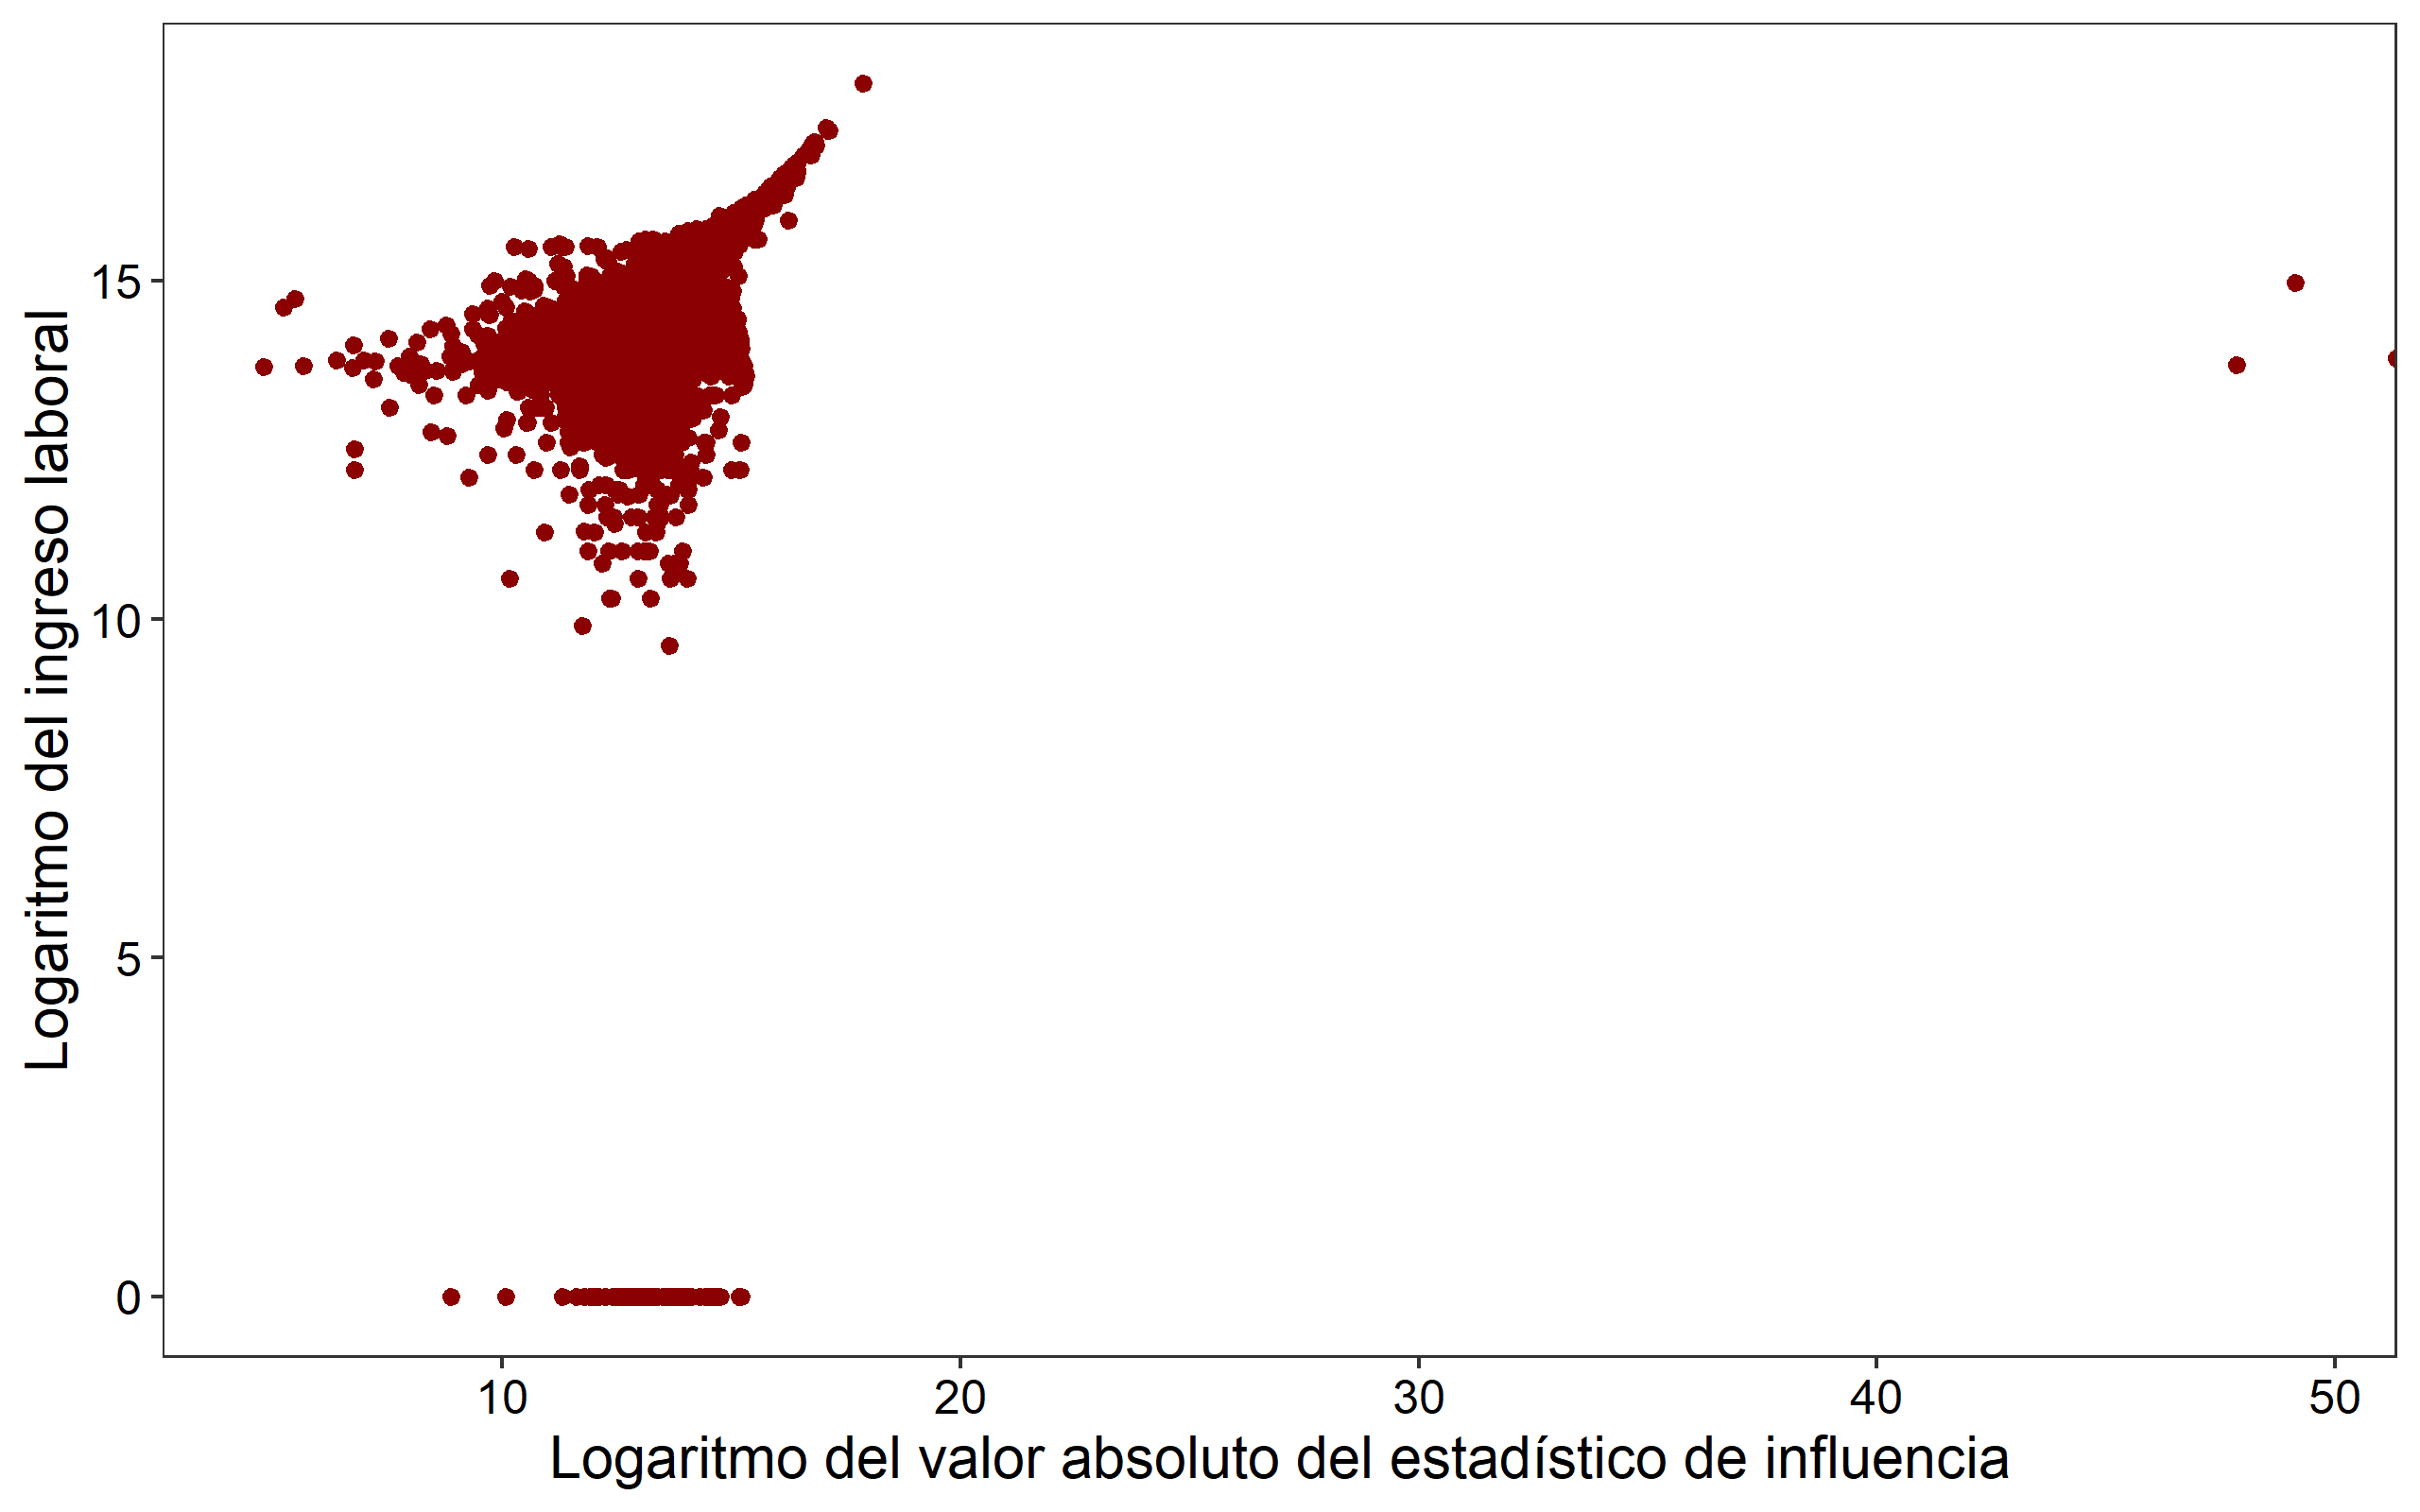
\includegraphics[width=\textwidth]{../views/analisis_influencia.png}
    \label{fig:influencia}
\end{figure}

A continuación se realiza el ejercicio de estimar el RMSE de los dos mejores modelos utilizando Leave One Out Cross Validation (LOOCV), el cual consiste en estimar los modelos para cada subconjunto posible de los datos tales que una de las observaciones quede por fuera de la muestra de entrenamiento. En el cuadro \ref{tbl:RMSELOOCV} se reporta el RMSE de los modelos 7 y 8 del cuadro \label{tbl:RMSEearnings} calculado por este método.


\begin{table}[H]
\centering
\caption{RMSE por LOOCV}
\label{tab:rmse_loocv}
\begin{tabular}{@{}ll@{}}
\toprule
Modelo & RMSE LOOCV \\ \midrule
7 & 234404932 \\ 
8 & 219100926 \\ \bottomrule
\end{tabular}
\label{tbl:RMSELOOCV}
\end{table}

Como puede observarse, el RMSE del modelo 8 es inferior al del modelo 7. No obstante, al compararlo con el RMSE del cuadro \label{tbl:RMSEearnings}, se observa que, para ambos modelos, el RMSE calculado por LOOCV es mayor. Como el RMSE calculado por LOOCV tiene menor sesgo es posible afirmar que el RMSE calculado usando el subconjunto de prueba subestima el verdadero RMSE. 


\bibliographystyle{apalike}
\bibliography{ref}


\end{document}
